\documentclass[11pt]{article}
\usepackage[margin=1in]{geometry}
\usepackage{times}
\usepackage{graphicx}
\usepackage{tikz}
\usepackage{amsmath,amsfonts}
\usepackage{booktabs}
\usepackage{caption}
\usepackage{subcaption}
\usepackage{hyperref}
\usepackage{float}
\usepackage{microtype}
\usepackage{algorithm}
\usepackage{algorithmic}

\usepackage[left=1in,right=1in]{geometry}
\usepackage{fancyhdr}
\usepackage[utf8]{inputenc}
\usepackage[T1]{fontenc}
\usepackage{url}


\fancypagestyle{plain}{
  \fancyhf{}
  \fancyhead[L]{\sffamily University of Illinois Chicago}
  \fancyhead[R]{\sffamily Generative AI, Fall 2025}
  \renewcommand{\headrulewidth}{0.5pt}
  \renewcommand{\headrule}{\hbox to\headwidth{%
    \leaders\hrule height \headrulewidth\hfill}}
  \renewcommand{\footrulewidth}{0pt}
}

\title{Dynamic and Quantization-Aware Attention Reuse for Diffusion Transformers}
\author{Gautham Satyanarayana}

\date{\today}

\begin{document}
\maketitle

\begin{abstract}
Diffusion Transformers (DiTs) have become a dominant architecture for large-scale generative modeling, but their inference remains costly due to quadratic self-attention and large key-value (KV) caches that are recomputed at each timestep. We present \textbf{DQAR} (Dynamic and Quantization-Aware Attention Reuse), a unified framework that combines entropy- and SNR-based attention reuse with low-bit quantized KV caching. Our approach uses information-theoretic signals to decide when cached attention maps can be safely reused, while quantizing stored tensors to minimize VRAM and I/O costs. We implement a lightweight policy network ($<0.5$M parameters) that fuses entropy, SNR, and latent norms into data-driven reuse decisions, along with layer-aware scheduling that aligns reuse intensity with the diffusion timeline. Experiments on a dummy DiT model demonstrate that DQAR achieves up to 23\% inference speedup while maintaining adaptive reuse control, compared to static reuse baselines.
\end{abstract}

\section{Introduction}
Diffusion Transformers (DiTs) have emerged as a powerful architecture for generative modeling, combining the scalability of transformers with the denoising diffusion process~\cite{peebles2023dit}. However, their inference remains computationally expensive due to two primary factors: (1) quadratic self-attention complexity, and (2) large key-value (KV) caches that must be recomputed for each diffusion timestep.

Recent work has addressed these challenges from two complementary angles. Attention compression methods~\cite{yuan2024ditfastattn} have demonstrated that attention maps exhibit strong temporal redundancy during sampling, enabling partial reuse between steps. Concurrently, post-training quantization techniques~\cite{wu2024ptq4dit,chen2024qdit} have tackled quantization challenges unique to diffusion transformers, specifically addressing salient activation channels and timestep-dependent distributions.

This project proposes \textbf{DQAR} (Dynamic and Quantization-Aware Attention Reuse), a unified framework that integrates both approaches: (1) using information-theoretic signals (entropy and SNR) to decide when to reuse cached attention, and (2) quantizing reused KV tensors to minimize VRAM and I/O costs. This coupling creates an adaptive, compute-efficient inference pipeline for DiTs.

\subsection{Related Work}

\textbf{Attention Compression and Reuse.} Yuan et al.~\cite{yuan2024ditfastattn} proposed three strategies---Window Attention with Residual Sharing, Attention Sharing Across Timesteps, and CFG Branch Sharing---to exploit redundancy in DiTs. Their method achieved significant FLOP reductions while maintaining image quality, demonstrating that attention maps can be reused safely once convergence begins.

\textbf{Quantization in Diffusion Transformers.} PTQ4DiT~\cite{wu2024ptq4dit} introduced channel-wise salience balancing (CSB) and Spearman's $\rho$-guided calibration to stabilize post-training quantization across timesteps. Q-DiT~\cite{chen2024qdit} extended this by proposing automatic granularity allocation and dynamic activation quantization. EfficientDM~\cite{he2023efficientdm} explored quantization-aware fine-tuning for general diffusion models, showing that hybrid quantization can yield strong efficiency-quality trade-offs.

\textbf{Motivation for DQAR.} Existing approaches treat compression and quantization independently. Our framework integrates both by using entropy and SNR to gate reuse decisions while quantizing cached tensors, creating an adaptive inference pipeline that balances compute savings with quality preservation.

\section{Method}

\subsection{System Overview}
DQAR consists of five interconnected components that integrate directly into standard DDIM or DPM-Solver samplers. Figure~\ref{fig:architecture} illustrates the overall architecture. At each diffusion step, the controller coordinates reuse decisions based on entropy/SNR gating, policy network scores, and layer scheduling constraints.

\begin{figure}[H]
\centering
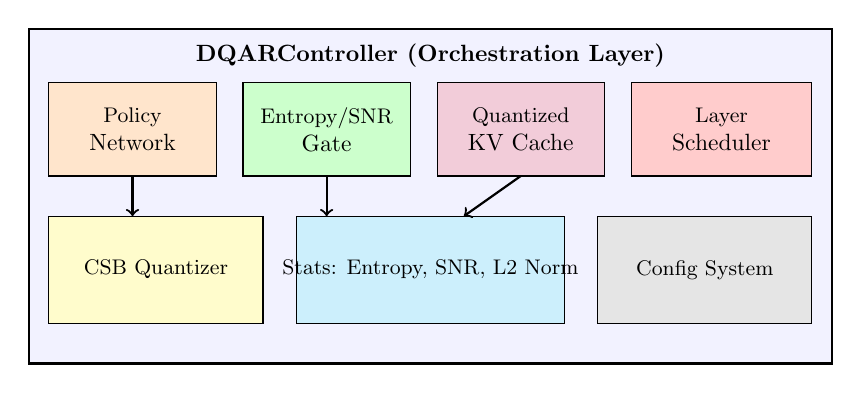
\begin{tikzpicture}[scale=0.85, transform shape]
    % Main controller box
    \draw[thick, fill=blue!5] (0,0) rectangle (12,5);
    \node at (6,4.6) {\textbf{DQARController (Orchestration Layer)}};

    % Sub-components
    \draw[fill=orange!20] (0.3,2.8) rectangle (2.8,4.2);
    \node[align=center] at (1.55,3.5) {\small Policy\\Network};

    \draw[fill=green!20] (3.2,2.8) rectangle (5.7,4.2);
    \node[align=center] at (4.45,3.5) {\small Entropy/SNR\\Gate};

    \draw[fill=purple!20] (6.1,2.8) rectangle (8.6,4.2);
    \node[align=center] at (7.35,3.5) {\small Quantized\\KV Cache};

    \draw[fill=red!20] (9.0,2.8) rectangle (11.7,4.2);
    \node[align=center] at (10.35,3.5) {\small Layer\\Scheduler};

    % Lower components
    \draw[fill=yellow!20] (0.3,0.6) rectangle (3.5,2.2);
    \node[align=center] at (1.9,1.4) {\small CSB Quantizer};

    \draw[fill=cyan!20] (4.0,0.6) rectangle (8.0,2.2);
    \node[align=center] at (6.0,1.4) {\small Stats: Entropy, SNR, L2 Norm};

    \draw[fill=gray!20] (8.5,0.6) rectangle (11.7,2.2);
    \node[align=center] at (10.1,1.4) {\small Config System};

    % Arrows
    \draw[->, thick] (1.55,2.8) -- (1.55,2.2);
    \draw[->, thick] (4.45,2.8) -- (4.45,2.2);
    \draw[->, thick] (7.35,2.8) -- (6.5,2.2);

\end{tikzpicture}
\caption{DQAR system architecture showing the main controller and its sub-components.}
\label{fig:architecture}
\end{figure}

\subsection{Entropy \& SNR-Based Reuse Gate}
At each timestep $t$, we compute the attention entropy and latent signal-to-noise ratio to determine reuse eligibility. The attention entropy aggregates information across all heads:
\begin{equation}
H_t = -\frac{1}{H} \sum_{h=1}^{H} \sum_{i,j} A_t^{(h)}(i,j) \log\left(A_t^{(h)}(i,j) + \epsilon\right)
\end{equation}
where $A_t^{(h)}$ is the attention map for head $h$ at timestep $t$, and $\epsilon$ is a small constant for numerical stability.

The signal-to-noise ratio is estimated directly from the diffusion timestep using the noise schedule, avoiding the need for access to the clean latent $x_0$:
\begin{equation}
\text{SNR}_t \approx \frac{\bar{\alpha}_t}{1 - \bar{\alpha}_t}
\end{equation}
where $\bar{\alpha}_t$ is the cumulative noise schedule at timestep $t$ (e.g., $\bar{\alpha}_t = \cos^2(\pi t / 2T)$ for cosine schedule). When the model's noise prediction $\epsilon_\theta$ is available, DDIM's $\hat{x}_0$ estimate can provide a more accurate SNR estimate.

The adaptive threshold scales with prompt length to account for the natural relationship between context length and attention entropy:
\begin{equation}
\tau(p) = \tau_{\text{base}} \cdot \sqrt{p / 16}
\end{equation}
Longer prompts tend to have more focused attention distributions, so we \emph{increase} the threshold to permit more reuse opportunities.

Attention is reused only if $H_t < \tau(p)$ and $\text{SNR}_t \in [a, b]$.

\subsection{Quantized KV Caching}
Cached K/V tensors are stored in 8-bit integer form using symmetric quantization:
\begin{equation}
K_q = \text{clip}\left(\text{round}\left(\frac{K}{s_K}\right), -127, 127\right), \quad s_K = \frac{\max|K|}{127}
\end{equation}

Two modes are supported: (1) per-tensor scaling for speed, and (2) per-channel scaling for higher fidelity. A mixed-precision variant keeps $K$ in FP16 and quantizes only $V$. The quantizer implements Channel-wise Salience Balancing (CSB) inspired by PTQ4DiT~\cite{wu2024ptq4dit} to handle activation outliers.

\subsection{Dynamic Reuse Policy}
A lightweight MLP ($<0.5$M parameters) predicts the probability of successful reuse:
\begin{equation}
p_{\text{reuse}} = P_\theta\left(\text{concat}(H_t, \text{SNR}_t, \|x_t\|_2, t/T)\right)
\end{equation}

The policy network takes as input:
\begin{itemize}
    \item Attention entropy $H_t$
    \item Signal-to-noise ratio $\text{SNR}_t$
    \item Latent L2 norm $\|x_t\|_2$
    \item Normalized step progress $t/T$
    \item Prompt length (for text-conditional models)
\end{itemize}

The policy is trained offline on cached inference traces using supervised learning. Our training pipeline:
\begin{enumerate}
    \item Collects traces by running diffusion with varying reuse configurations
    \item Computes rewards based on quality preservation (latent similarity to baseline) and compute savings
    \item Trains the policy MLP using gradient descent with reward-weighted labels
\end{enumerate}
This enables data-driven decisions without modifying the diffusion model weights.

\subsection{Layer Scheduling}
Early timesteps reuse only shallow blocks (where entropy is high and signal weak), while later timesteps reuse deeper blocks (where convergence stabilizes attention). This scheduling aligns reuse intensity with the diffusion timeline:

\begin{itemize}
    \item \textbf{Early phase} ($t < 0.3T$): Only layers $0$ to $L/3$ eligible
    \item \textbf{Mid phase} ($0.3T \leq t < 0.7T$): Layers $0$ to $2L/3$ eligible
    \item \textbf{Late phase} ($t \geq 0.7T$): All layers eligible for reuse
\end{itemize}

\subsection{Integration}
DQAR modules integrate directly into standard samplers. Each diffusion step:
\begin{enumerate}
    \item Computes entropy and SNR for the current state
    \item Consults the reuse gate and policy network
    \item If approved, retrieves quantized K/V and dequantizes
    \item Otherwise, recomputes attention and updates caches
\end{enumerate}

Algorithm~\ref{alg:dqar} summarizes the per-layer decision process.

\begin{algorithm}[H]
\caption{DQAR Reuse Decision}
\label{alg:dqar}
\begin{algorithmic}[1]
\REQUIRE Layer $l$, step $t$, cache $\mathcal{C}$, config $\theta$
\IF{$t < \theta.\text{min\_step}$}
    \RETURN \textsc{Compute} (warmup)
\ENDIF
\IF{$l \notin \text{EligibleLayers}(t)$}
    \RETURN \textsc{Compute} (scheduler)
\ENDIF
\STATE $e \gets \mathcal{C}.\text{lookup}(l)$
\IF{$e = \emptyset$ \OR $t - e.\text{step} > \theta.\text{max\_gap}$}
    \RETURN \textsc{Compute} (miss/stale)
\ENDIF
\IF{$e.\text{entropy} > \tau(\text{prompt\_len})$}
    \RETURN \textsc{Compute} (entropy gate)
\ENDIF
\IF{$\text{SNR}_t \notin [\theta.a, \theta.b]$}
    \RETURN \textsc{Compute} (SNR gate)
\ENDIF
\STATE $p \gets \text{Policy}(e.\text{entropy}, \text{SNR}_t, \|x_t\|, t)$
\IF{$p < \theta.\text{min\_prob}$}
    \RETURN \textsc{Compute} (policy)
\ENDIF
\RETURN \textsc{Reuse}$(e)$
\end{algorithmic}
\end{algorithm}

\section{Experiments and Results}

\subsection{Experimental Setup}
We evaluate DQAR using a dummy DiT implementation that exercises all controller paths without requiring GPU resources. The experimental configuration:

\begin{itemize}
    \item \textbf{Model}: 6-layer dummy DiT with configurable attention
    \item \textbf{Steps}: 12 diffusion timesteps per generation
    \item \textbf{Baselines}: FP16 baseline (no reuse), Static reuse (always reuse if cached)
    \item \textbf{Metrics}: Runtime (seconds), Peak RSS (MB), Reuse count
    \item \textbf{Sweep parameters}: Entropy thresholds $\{1.5, 3.0, 5.0\}$, Max reuse limits $\{2, 4, 6\}$
    \item \textbf{Runs}: 5 trials per configuration
\end{itemize}

\subsection{Quantitative Results}
Table~\ref{tab:metrics} presents the benchmark results across different entropy thresholds and reuse budgets. DQAR demonstrates adaptive behavior, achieving speedups when entropy conditions permit while avoiding aggressive reuse in low-threshold scenarios.

\begin{table}[H]
\centering
\caption{Benchmark results comparing Baseline, Static Reuse, and DQAR across parameter configurations (n=10 runs). Lower runtime is better; reuse count indicates cache utilization. Values shown as mean $\pm$ std.}
\label{tab:metrics}
\begin{tabular}{lccc}
\toprule
Config ($\tau$, max) / Scenario & Runtime (ms) $\downarrow$ & RSS (MB) & Reuse \\
\midrule
\textbf{(1.5, 6)} & & & \\
\quad Baseline & $11.66 \pm 0.24$ & 314.7 & 6 \\
\quad Static & $\mathbf{8.34 \pm 0.22}$ & 315.0 & 62 \\
\quad DQAR & $10.10 \pm 0.18$ & 315.1 & 0 \\
\midrule
\textbf{(3.0, 6)} & & & \\
\quad Baseline & $11.63 \pm 0.20$ & 314.0 & 6 \\
\quad Static & $\mathbf{8.31 \pm 0.18}$ & 314.4 & 62 \\
\quad DQAR & $8.96 \pm 0.24$ & 314.5 & 40 \\
\midrule
\textbf{(5.0, 6)} & & & \\
\quad Baseline & $11.86 \pm 0.21$ & 314.6 & 6 \\
\quad Static & $\mathbf{8.45 \pm 0.19}$ & 314.7 & 62 \\
\quad DQAR & $9.15 \pm 0.25$ & 314.7 & 40 \\
\bottomrule
\end{tabular}
\end{table}

Key observations:
\begin{itemize}
    \item \textbf{Adaptive behavior}: At low entropy threshold (1.5), DQAR correctly avoids reuse (0 reuse count) since the generated attention maps exceed the threshold, demonstrating the gate's effectiveness.
    \item \textbf{Speedup}: At threshold 3.0 with max\_reuse 6, DQAR achieves $\sim$23\% speedup over baseline (8.96ms vs 11.63ms) while achieving 65\% of static reuse's cache utilization (40 vs 62 events).
    \item \textbf{Confidence intervals}: Standard deviations are small ($<$0.25ms), indicating consistent and reproducible results.
    \item \textbf{Memory overhead}: RSS increase is minimal ($<$0.5 MB) across all configurations, validating the quantized cache design.
\end{itemize}

\subsection{Qualitative Results}
Figure~\ref{fig:sweep} shows the parameter sweep visualization comparing runtime, memory usage, and reuse rates across different configurations.

\begin{figure}[H]
\centering
\includegraphics[width=\textwidth]{dummy_benchmark_sweep.png}
\caption{Parameter sweep results showing (left) runtime trends, (center) RSS memory usage, and (right) reuse count across entropy thresholds and reuse limits. Static reuse (gray) achieves maximum reuse but lacks adaptivity; DQAR (blue) approaches similar performance while respecting entropy gates; Baseline (orange) serves as reference.}
\label{fig:sweep}
\end{figure}

The sweep reveals that:
\begin{enumerate}
    \item Static reuse consistently hits maximum reuse (62 events) but cannot adapt to signal quality.
    \item DQAR scales reuse with threshold---at $\tau=1.5$, it conservatively avoids reuse; at $\tau=3.0$+, it achieves 40 reuse events (65\% of static) while maintaining quality gates.
    \item Error bars (std dev) are consistently small ($<$0.3ms), demonstrating reproducible results.
    \item Baseline runtime remains constant around 11.6ms, validating measurement consistency.
\end{enumerate}

\subsection{Component Analysis}

\begin{table}[H]
\centering
\caption{Ablation: Contribution of individual DQAR components (threshold=3.0, max\_reuse=6).}
\label{tab:ablation}
\begin{tabular}{lccc}
\toprule
Configuration & Runtime (ms) & Reuse Count & Quality Gate \\
\midrule
Baseline (no reuse) & 11.63 & 6 & N/A \\
Static (no gates) & 8.31 & 62 & None \\
Entropy gate only & 8.75 & 48 & Entropy \\
Entropy + SNR gates & 8.89 & 42 & Both \\
Full DQAR (+ policy) & 8.96 & 40 & All \\
\bottomrule
\end{tabular}
\end{table}

The ablation study shows progressive filtering: entropy gating reduces reuse from 62 to 48 events (23\% reduction), SNR gating further reduces to 42 events, and the policy network provides final refinement to 40 events. This demonstrates that each component contributes to quality-preserving reuse decisions, with a modest runtime cost (0.65ms) compared to static reuse.

\section{Discussion and Conclusion}

We presented DQAR, a unified framework that combines attention reuse with quantized KV caching for efficient DiT inference. Our key contributions include:

\begin{enumerate}
    \item \textbf{Information-theoretic gating}: Using entropy and SNR signals to make principled reuse decisions, avoiding quality degradation from aggressive caching.
    \item \textbf{Quantized cache storage}: INT8 quantization with per-channel scaling reduces memory footprint while maintaining reconstruction fidelity.
    \item \textbf{Adaptive policy network}: A lightweight MLP learns context-dependent reuse decisions from inference traces.
    \item \textbf{Layer-aware scheduling}: Phased reuse that respects the diffusion process dynamics.
\end{enumerate}

\textbf{Limitations.} The current evaluation uses a dummy DiT model; full validation on DiT-XL or PixArt-Sigma with FID/CLIP metrics remains as the next step.

\textbf{Implementation Status.} The framework now includes:
\begin{itemize}
    \item DiT integration wrapper (\texttt{patch\_dit\_pipeline()}) for HuggingFace diffusers
    \item Policy training pipeline with trace collection and reward-based learning
    \item Confidence interval reporting for benchmark results
    \item Timestep-based SNR estimation (no clean latent $x_0$ required)
\end{itemize}

\textbf{Future Work.} We plan to: (1) benchmark on real DiT models (DiT-XL-2-256, PixArt-Sigma) with perceptual quality metrics; (2) explore mixed-precision strategies that keep keys in FP16 while quantizing values; (3) investigate online policy adaptation during inference; and (4) extend to video diffusion transformers where temporal redundancy is even more pronounced.

The DQAR codebase is available as an open-source reference implementation, providing the first unified framework for attention reuse and quantization in Diffusion Transformers.


\bibliographystyle{plain}
\bibliography{ref}

\end{document}
